\chapter{计算机网络体系结构}\label{CN01}

\section{网络组成、分类与拓扑}\label{CN01-network}

计算机网络将具有独立功能的计算设备通过链路和网络设备连接，按共同协议实现数据通信、资源共享和分布式处理。

\par\smallskip
{\fontsize{9.3}{12}\selectfont\setlength{\tabcolsep}{2.5pt}\setlength{\LTleft}{0pt}\setlength{\LTright}{0pt}
\begin{longtable}{@{}>{\raggedright\arraybackslash}p{\dimexpr0.28571\linewidth-2\tabcolsep\relax}>{\raggedright\arraybackslash}p{\dimexpr0.71429\linewidth-2\tabcolsep\relax}@{}}
\toprule
分类依据 & 划分及含义 \\

\midrule\endfirsthead\toprule
分类依据 & 划分及含义 \\

\midrule\endhead\bottomrule\endfoot
工作方式 & 边缘：端系统与应用；核心：互联网络和转发设备 \\

功能 & 资源子网：计算、存储与共享资源；通信子网：数据传送 \\

覆盖范围 & PAN、LAN、MAN、WAN；名称没有统一公里数界限 \\

传输方式 & 广播式：多站共享介质；点到点式：链路连接两端 \\

其他维度 & 公用/专用、有线/无线，可独立组合 \\

\end{longtable}}
\par\smallskip

internet 泛指网络互连；Internet 指采用 TCP/IP 协议族的全球互联网。ISP 提供互联网接入等服务。网络组成包括硬件、软件和协议。服务复制可提高可用性，还须配合故障检测和一致性机制。

总线、星形、环形、网状描述连接关系。集线器组成物理星形、逻辑共享介质；交换机星形各端口可并行。路径由多段链路组成：H1---R1---R2---H2 有3段链路、2个中间节点。

\section{速率、吞吐量与时延}\label{CN01-delay}

速率单位 bit/s，数据单位换算为 \(1\mathrm{B}=8\mathrm{bit}\)；\(\mathrm{k},\mathrm{M},\mathrm{G}\) 分别为 \(10^3,10^6,10^9\)，二进制量使用 KiB、MiB 或题设约定。

\par\smallskip
\begin{wideblock}
{\fontsize{9.3}{12}\selectfont\setlength{\tabcolsep}{2.5pt}\setlength{\LTleft}{0pt}\setlength{\LTright}{0pt}
\begin{longtable}{@{}>{\raggedright\arraybackslash}p{\dimexpr0.24716\linewidth-2\tabcolsep\relax}>{\raggedright\arraybackslash}p{\dimexpr0.37074\linewidth-2\tabcolsep\relax}>{\raggedright\arraybackslash}p{\dimexpr0.38210\linewidth-2\tabcolsep\relax}@{}}
\toprule
指标 & 公式或定义 & 使用条件 \\

\midrule\endfirsthead\toprule
指标 & 公式或定义 & 使用条件 \\

\midrule\endhead\bottomrule\endfoot
发送时延 & \(t_{tx}=L/R\) & 从首比特进入链路至末比特进入；\(L\) 用 bit \\

传播时延 & \(t_{prop}=d/v\) & 同一比特走完链路；距离与速度单位统一 \\

单跳完整接收时间 & \(L/R+d/v\) & 无排队、处理开销 \\

总时延 & 各跳发送、传播、处理、排队按事件累加 & 流水重叠部分只计一次 \\

时延带宽积 & \(R t_{prop}\) & 单向传播中可容纳的比特数 \\

往返在途量 & \(R\cdot RTT\) & 为覆盖反馈等待估计所需窗口 \\

\end{longtable}}
\end{wideblock}
\par\smallskip

带宽在性能题中常指额定速率；吞吐量是观察期间实际通过的数据率；有效吞吐量只计有效载荷。路径单流长期吞吐量不超过最慢链路速率，竞争和协议开销会继续降低它。

RTT须读清计时边界。题给往返传播时延时，数据与确认的发送时间另计；给出实际请求响应时间时，按题意避免重复累加。信道利用率按题设确定分子，可指忙时比例，也可特指发送有效数据所占比例。

理想排队模型 \(D=D_0/(1-U)\) 仅用于给定模型：\(D_0\)为空闲时延，\(U\)为归一化利用率。独立比特误码概率为 \(p\)、帧长为 \(L\) bit 时，帧错概率 \(1-(1-p)^L\)；\(pL\ll1\) 时近似 \(pL\)，突发错误不能直接沿用此模型。

\section{协议、服务、接口与封装}\label{CN01-layers}

\par\smallskip
{\fontsize{9.3}{12}\selectfont\setlength{\tabcolsep}{2.5pt}\setlength{\LTleft}{0pt}\setlength{\LTright}{0pt}
\begin{longtable}{@{}>{\raggedright\arraybackslash}p{\dimexpr0.28051\linewidth-2\tabcolsep\relax}>{\raggedright\arraybackslash}p{\dimexpr0.71949\linewidth-2\tabcolsep\relax}@{}}
\toprule
概念 & 约束关系与内容 \\

\midrule\endfirsthead\toprule
概念 & 约束关系与内容 \\

\midrule\endhead\bottomrule\endfoot
协议 & 对等实体的水平规则；语法规定格式，语义规定含义和动作，时序规定事件次序 \\

服务 & 本层与下层协作后向上层提供的能力 \\

接口、SAP & 同机相邻层使用服务的方式、服务访问位置 \\

体系结构 & 规定分层、功能及相互关系；内部算法和数据结构由实现选择 \\

\end{longtable}}
\par\smallskip

服务原语描述同机层间事件：请求、指示，以及需应答时的响应、证实。一次原语可引起多次协议报文、超时或重试。

\(n\)层PDU由控制信息PCI和服务数据SDU封装：\(n\text{-PDU}=n\text{-PCI}+n\text{-SDU}\)。上层PDU成为下层SDU；PCI可位于首部或尾部。接收端逐层解封装，对等通信依靠本机下层实际传送。

\begin{figure}[H]
\centering
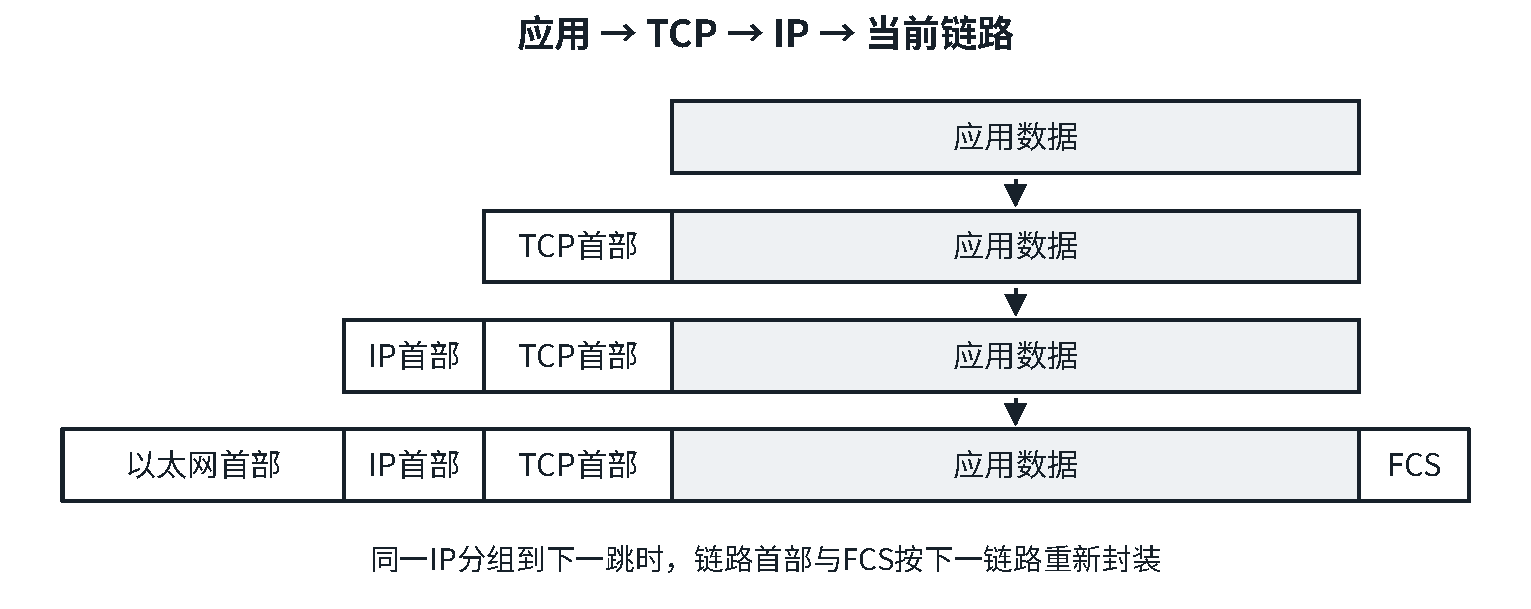
\includegraphics[width=\linewidth,height=108mm,keepaspectratio]{figures/CN01_encapsulation.pdf}
\caption{逐层封装与链路层当前一跳}\label{cn-fig-encapsulation}
\end{figure}

\par\smallskip
{\fontsize{9.3}{12}\selectfont\setlength{\tabcolsep}{2.5pt}\setlength{\LTleft}{0pt}\setlength{\LTright}{0pt}
\begin{longtable}{@{}>{\raggedright\arraybackslash}p{\dimexpr0.21466\linewidth-2\tabcolsep\relax}>{\raggedright\arraybackslash}p{\dimexpr0.34279\linewidth-2\tabcolsep\relax}>{\raggedright\arraybackslash}p{\dimexpr0.44254\linewidth-2\tabcolsep\relax}@{}}
\toprule
标识 & 所属层及长度 & 普通跨路由转发 \\

\midrule\endfirsthead\toprule
标识 & 所属层及长度 & 普通跨路由转发 \\

\midrule\endhead\bottomrule\endfoot
MAC & 链路层，以太网48 bit & 每跳重新封装，目的为当前下一跳接口 \\

IP & 网络层，IPv4为32 bit & 无NAT时源、目的通常保持 \\

端口 & 传输层，16 bit & 无端口转换时保持，用于进程端点分用 \\

\end{longtable}}
\par\smallskip

面向连接服务通常先建立、再传送、后释放；无连接服务独立提交数据单元。可靠交付、是否确认、是否预留资源分别由协议规定。以太网CRC只检错；802.11单播ACK只确认当前无线跳；端到端可靠性由端系统协议保障。

\section{OSI与TCP/IP功能对应}\label{CN01-models}

\par\smallskip
\begin{wideblock}
{\fontsize{9.3}{12}\selectfont\setlength{\tabcolsep}{2.5pt}\setlength{\LTleft}{0pt}\setlength{\LTright}{0pt}
\begin{longtable}{@{}>{\raggedright\arraybackslash}p{\dimexpr0.19415\linewidth-2\tabcolsep\relax}>{\raggedright\arraybackslash}p{\dimexpr0.45531\linewidth-2\tabcolsep\relax}>{\raggedright\arraybackslash}p{\dimexpr0.35054\linewidth-2\tabcolsep\relax}@{}}
\toprule
OSI层次 & 对象与主要功能 & TCP/IP对应 \\

\midrule\endfirsthead\toprule
OSI层次 & 对象与主要功能 & TCP/IP对应 \\

\midrule\endhead\bottomrule\endfoot
应用 & Web、邮件、名称服务等应用功能 & 应用层 \\

表示 & 表示转换、压缩、加密 & 应用层 \\

会话 & 对话管理、同步与恢复 & 应用层 \\

传输 & 进程端到端复用分用；按协议提供可靠性、流控 & TCP、UDP \\

网络 & 跨网络分组寻址、路由和转发 & 网际层IP，尽最大努力数据报 \\

数据链路 & 相邻节点成帧、检错、介质访问；可含流控和重传 & 网络接口层 \\

物理 & 原始比特、电平、编码和接口 & 网络接口层 \\

\end{longtable}}
\end{wideblock}
\par\smallskip

五层教学模型把网络接口层展开为数据链路层和物理层。流控所属层由控制范围决定：相邻节点用链路层，应用进程端到端用传输层。具体协议是否实现某项功能，须查该协议提供的服务。

\par\medskip\Needspace{4\baselineskip}\noindent\hypertarget{CN01-E01}{}\label{CN01-E01}\textbf{例 1-1}\par\nobreak\smallskip

在 OSI 参考模型中，自下而上第一个提供端到端服务的层次是（　）。

A. 数据链路层　B. 传输层　C. 会话层　D. 应用层

\par\medskip\Needspace{4\baselineskip}\noindent\hypertarget{CN01-E02}{}\label{CN01-E02}\textbf{例 1-2}\par\nobreak\smallskip

在 ISO/OSI 参考模型中，实现两个相邻结点间流量控制功能的是（　）。

A. 物理层　B. 数据链路层　C. 网络层　D. 传输层

\section{交换方式与存储转发计算}\label{CN01-switching}

\par\smallskip
\begin{wideblock}
{\fontsize{9.3}{12}\selectfont\setlength{\tabcolsep}{2.5pt}\setlength{\LTleft}{0pt}\setlength{\LTright}{0pt}
\begin{longtable}{@{}>{\raggedright\arraybackslash}p{\dimexpr0.18980\linewidth-2\tabcolsep\relax}>{\raggedright\arraybackslash}p{\dimexpr0.35508\linewidth-2\tabcolsep\relax}>{\raggedright\arraybackslash}p{\dimexpr0.45512\linewidth-2\tabcolsep\relax}@{}}
\toprule
方式 & 转发条件 & 主要时间和资源代价 \\

\midrule\endfirsthead\toprule
方式 & 转发条件 & 主要时间和资源代价 \\

\midrule\endhead\bottomrule\endfoot
电路交换 & 先建立电路，再连续传送比特流 & 建立时间、源端发送、全程传播；空闲时可仍占资源 \\

报文交换 & 中间节点收全整份报文后转发 & 长报文逐跳发送与缓存 \\

分组交换 & 存储转发时收全一组再转发 & 分组首部、处理、排队；可跨链路流水 \\

\end{longtable}}
\end{wideblock}
\par\smallskip

固定路径含 \(h\) 段等速链路，\(n\)个等长分组，每组总长 \(L\) bit、速率 \(R\)，无竞争和处理开销时：

\[T=(n+h-1)\frac LR+\sum_{i=1}^h t_{prop,i}.\]

第一组完成需 \(hL/R+\sum t_{prop,i}\)，后续每组间隔 \(L/R\)。报文长 \(F\) bit，整报文存储转发发送项为 \(hF/R\)；已建立理想电路发送项为 \(F/R\)，再加传播及题给开销。

\begin{figure}[H]
\centering
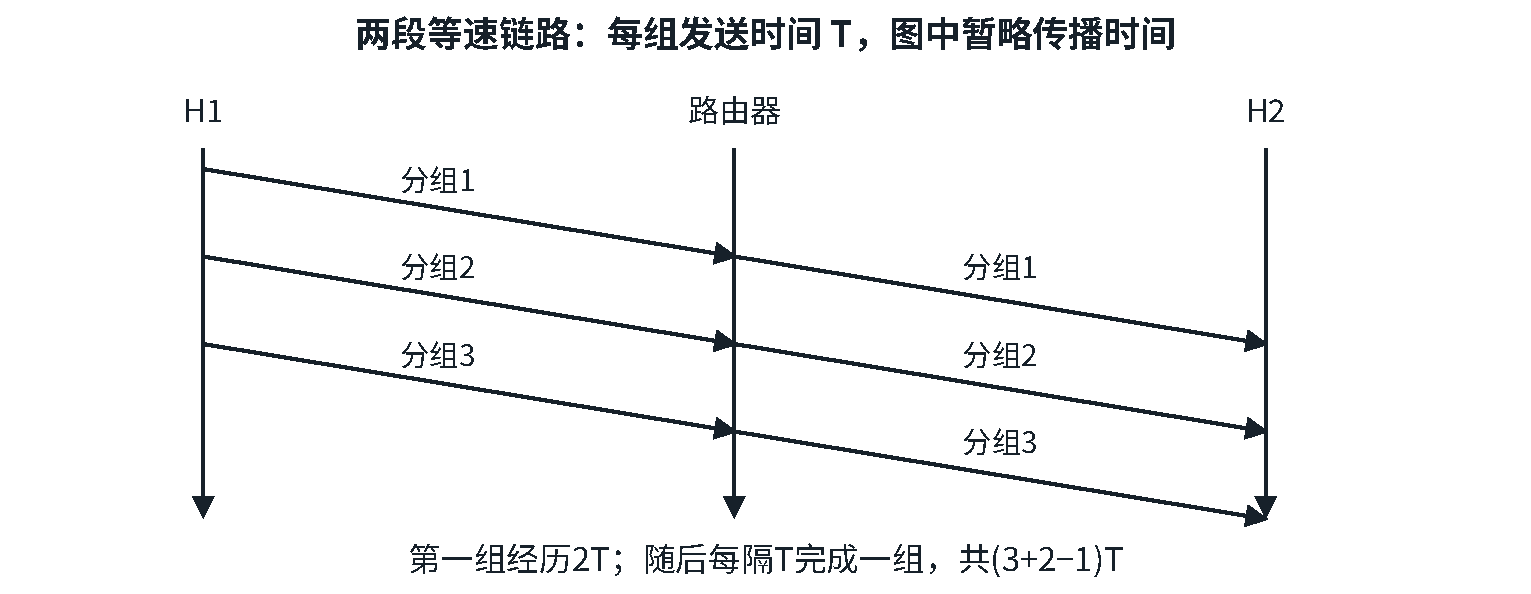
\includegraphics[width=\linewidth,height=108mm,keepaspectratio]{figures/CN02_packet_pipeline.pdf}
\caption{等速链路上的分组流水}\label{cn-fig-pipeline}
\end{figure}

异速、变长、含处理时延时用事件递推。令 \(F_{i,j}\) 为第\(j\)组在链路\(i\)发送完的时刻，\(p_{i-1,j}\)为上一节点收到后处理时间：

\[F_{i,j}=\max\{F_{i,j-1},\ F_{i-1,j}+t_{prop,i-1}+p_{i-1,j}\}+L_j/R_i.\]

源端准备时刻作边界条件；目的收齐时间为 \(F_{h,n}+t_{prop,h}\)。若处理器串行且会排队，另记录处理器空闲时刻。

\par\medskip\Needspace{4\baselineskip}\noindent\hypertarget{CN01-E03}{}\label{CN01-E03}\textbf{例 1-3}\par\nobreak\smallskip

在下图所示的分组交换网络中，主机 H1 和 H2 通过路由器互连，2段链路的带宽均为100 Mb/s，时延带宽积（即单向传播时延\ensuremath{\times}带宽）均为1000 bit。若 H1 向 H2 发送1个大小为1 MB的文件，分组长度为1000 B，则从 H1 开始发送时刻起到 H2 收到文件全部数据时刻止，所需的时间至少是（注：\(M=10^6\)）（　）。

\begin{figure}[H]
\centering
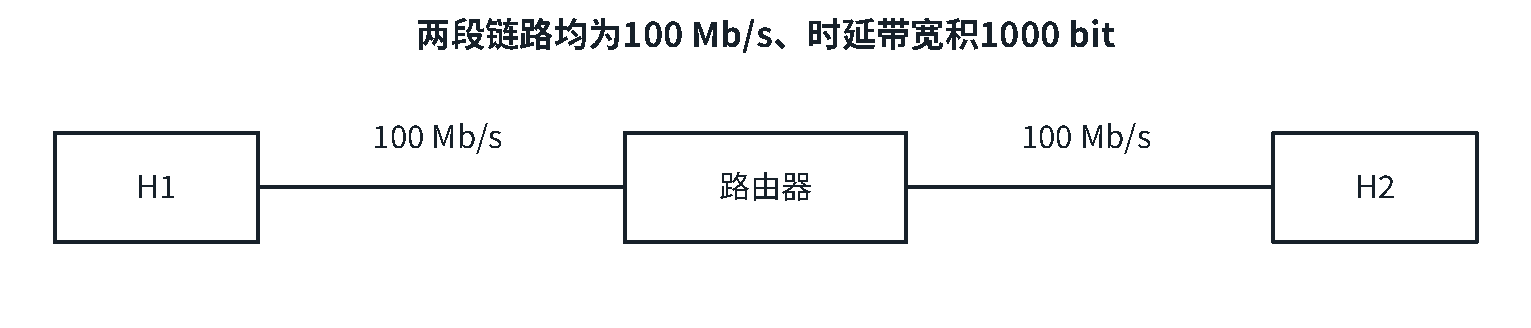
\includegraphics[width=\linewidth,height=108mm,keepaspectratio]{figures/CN15_two_links_2023.pdf}
\caption{原题的两段链路，均为100 Mb/s且时延带宽积1000 bit}\label{cn-fig-2023links}
\end{figure}

A. 80.02 ms　B. 80.08 ms　C. 80.09 ms　D. 80.10 ms

\section{数据报与虚电路}\label{CN01-datagram-vc}

\par\smallskip
{\fontsize{9.3}{12}\selectfont\setlength{\tabcolsep}{2.5pt}\setlength{\LTleft}{0pt}\setlength{\LTright}{0pt}
\begin{longtable}{@{}>{\raggedright\arraybackslash}p{\dimexpr0.22119\linewidth-2\tabcolsep\relax}>{\raggedright\arraybackslash}p{\dimexpr0.38312\linewidth-2\tabcolsep\relax}>{\raggedright\arraybackslash}p{\dimexpr0.39569\linewidth-2\tabcolsep\relax}@{}}
\toprule
比较项 & 数据报 & 虚电路 \\

\midrule\endfirsthead\toprule
比较项 & 数据报 & 虚电路 \\

\midrule\endhead\bottomrule\endfoot
准备与路由 & 无预建逐跳连接；各分组独立选路 & 建立时选路并保存状态 \\

转发依据 & 分组目的地址 & 输入链路和局部VCID映射 \\

顺序 & 路径可不同，可乱序 & 通常沿既定路径，保持顺序 \\

链路资源 & 分组动态共享 & 仍可动态共享，保障由具体服务规定 \\

\end{longtable}}
\par\smallskip

VCID可逐跳变化；永久虚电路可长期保留。虚电路的逻辑连接与电路交换的专用资源分配分别判断。

\par\medskip\Needspace{4\baselineskip}\noindent\hypertarget{CN01-E04}{}\label{CN01-E04}\textbf{例 1-4}\par\nobreak\smallskip

下列关于虚电路网络的叙述中，错误的是（　）。

A. 可以确保数据分组传输顺序

B. 需要为每条虚电路预分配带宽

C. 建立虚电路时需要进行路由选择

D. 依据虚电路号（VCID）进行数据分组转发
